\chapter{Development of the Artefact}\label{ch3}

The problem of StyleGAN generated faces aiding in the malicious creation of false identities confirmed in the crackdown of Facebook profiles as shown by \cite{Chandler2016} and in the new addition of StyleGAN3 where the creator Nvidea also emphasized the problem and research aiming to detect these images \citep{Karras2021}.

In this projects literature study it was identified that a machine learning deep neural network approach will be the simplest solution to the problem. A neural network that can identify images as either real human images or images generated by StyleGAN with relative accuracy as a method for detection must be implemented in an easy to use front end for the aims of this project to be satisfied. The proposed method of detection should be the easiest solution to the problem as substantiated by \cite{rasmussen2001} with their findings concluding that a simple neural network is usually the best neural network.

\section{Artefact Description}

The artefact for this proposed project can be divided into two main aspects namely the neural network model that will train on 2 separate datasets to classify new images between the characteristics of the data classes it learned in trained. The second aspect is the minimal front-end that will allow users to easily interact with the neural network model and receive simple output on the identification of their uploaded images. The neural network was created using the python programming language in a Jupyter notebook that was compiled and executed on the Google Colab virtual cloud-based environment. To create the neural network popular machine learning packages in the python language was used namely Keras and TensorFlow. The neural network was evaluated and determined to be sufficient, but improvisations could be made using the new technology Optuna for hyperparameter optimization. The neural network was then implemented in a minimalistic front end web app using the python web framework Flask.

\section{Artefact Life Cycle}

The development of the artefact was conducted with the use of DSRM and an Agile combination as stated in  Chapter \ref{ch1}. The DSRM  

\section{Description of the Development of the Artefact}

As stated in the methodologies used in Chapter \ref{ch1} and the Artefact Life Cycle the development of the artefact in this project was subdivided into Sprints. Each sprint handled a subset of tasks to allow for a manageable section of development. This partitioning of the overall workload aided in the development of the artefact and the subsequent testing of the implementations to ultimately ensure a successful project compared to the initial project aims and objectives. Therefore the overall artefact development will be discussed in terms of these sprints. The software used and implemented as well as the final implementation of the method of detection will be structured out in these sprints. 

\section{Sprints}

In the development of the artefact, the overall workload was subdivided into 4 separate sprints. In the 1\textsuperscript{St} Sprint the datasets were retrieved and compiled and an initial neural network was created. The 2\textsuperscript{Nd} Sprint entailed training the neural network and evaluating the accuracy of the model in detecting StyleGAN generated images. The 3\textsuperscript{Rd} Sprint used the results of the evaluation in the 2\textsuperscript{Nd} Sprint and it was determined that improvements could be made. Optuna was used to improve the neural network model. The 4\textsuperscript{Th} and final sprint completed the method of detection by implementing the neural network into a minimalistic front-end web application using the Flask framework.

\subsection{Sprint 1}

In the 1\textsuperscript{St} Sprint of the development of the artefact the StyleGAN dataset was downloaded from the official StyleGAN GitHub repository where various datasets are included of StyleGAN generated images. For the images of real human faces, the FlickrFaces dataset was retrieved from the FlickrFaces GitHub repository. The original datasets contained 100 000 images each and for the detection of StyleGAN images, a subset was created of these datasets that reduced them in size by the number of images and included them together in a dataset that can be used in the training of the neural network model \citep{Karras2019}.

\subsubsection{Downloading and the Dataset}

The datasets that are provided by StyleGAN and the FlickrFaces dataset each contain 100 000 high-quality images. The problem however that was faced is that these high-quality image datasets were also very large. Conventionally datasets used and sometimes contained in software such as Google Colab and Kaggle is small in total size. The StyleGAN high quality generated faces image dataset size was a total of 175GB and the FlickrFaces dataset total size was 140GB. 

The two datasets were made available on their respective GitHub repositories, redirecting to the file buckets hosted in Google Drive. To access the data locally the drives were shared to an NWU institution Google Drive account which does not have a storage limit. In Google Drive shortcuts to the original datasets could be added to the home directory of the account. the datasets could then be downloaded from the home directory.

The problem however faced when using this method is the internet limitations posed on campus at the North-West University's Potchefstroom campus. When downloading through a browser using on-campus internet infrastructure the connection will be throttled if a single file larger than 1GB is downloaded. Google Drive automatically compresses downloads into zip files when downloading and individual files cannot be downloaded sequentially using the internet browsers. Speeds up until 1GB downloaded would stay constant and at high-capacity then after reaching 1GB would be throttled down to low inconsistent speeds. A better way to retrieve the datasets locally had to be used.

\begin{figure}[H]%
\centering
\fbox{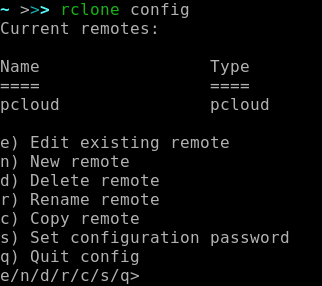
\includegraphics[width=0.5\textwidth]{img/f10rclone.png}}%
\caption{rclone setup config example \citep{rclone2021}}%
\label{fig:10}%
\end{figure}

To address the problem of internet speeds being throttled when downloading the datasets the command-line software rclone was used. rclone, a Linux native package, was installed on the windows local system using the dedicated windows installer. As demonstrated in Figure \ref{fig:10} rclone could be opened up in the command line and after mounting a connection to the Google Drive account could the whole dataset be downloaded sequentially. Each file is downloaded individually from the Google Drive dataset to the local machine, and the total download times of both datasets are completed overnight.

\subsubsection{Dataset Preparation}

The datasets had to be compiled together into one dataset that was used within training the neural network. When training a neural network for a binary image classification problem the dataset directory structure is an important aspect of the data. When the neural network trains and validates its training it compares its prediction with the original image file directory in both training and validation. If the network predicts an image to be StyleGAN generated it checks its prediction against the folder in which the file is located. The subdirectories for the datasets created in this project followed a similar structure to that of the Cat-vs-Dog problem that is used when learning about binary image classifications in neural networks. Table \ref{tabl:folders} shows the structure of the dataset, this directory structure remained the same for all subsequent datasets as they were created to address the resources problems that were identified in Sprint 2 and for the hyperparameter optimization trails in Sprint 3.

\begin{table}[H]%
\caption{Folder Structure of the dataset used in identifying StyleGAN images}
\label{tabl:folders}
\center
\small
\fbox{
  \begin{forest}
    for tree={font=\sffamily, %grow'=0,
    folder indent=.9em, folder icons,
    edge=densely dotted}
    [\textbf{Dataset}
      [train, this folder size=20pt
          [ff]
          [sg]]
      [valid, this folder size=20pt
          [ff]
          [sg]]
      [test, this folder size=20pt
          [ff]
          [sg]]    
      [\textit{vectorize.py}, is file]
    ]
  \end{forest}
  }
\end{table}

Initially, the subset created from the StyleGAN and FlickrFaces datasets retrieved consisted of 20 000 images. The number of images used for the identification of StyleGAN images was decided based on the findings of \cite{Nasr2016}, that concluded the more images a neural network can use in image classification the better its prediction will be. To an extent, this is true for the problem of StyleGAN generated images versus images of real human faces due to the fine differences between the two types of images. The neural network won't classify the images based on the shape as in the Cat-vs-Dog problem but will rather focus on the small artefacts or features that are present in StyleGAN images for its classification. 

Using too large a dataset can lead to the neural network overfitting the data \citep{Trask2019}. Overfitting occurs when the created neural network model becomes exceptionally good at being classifying the dataset it trained on, but performs much worse when classifying data that it was not trained on. Because of the scope of the proposed project the neural network that is created does not have to be the "\textit{perfect}" model, and will in a sense overfit facial recognition features as that is the premise for the creation of the model. What this means is that if the model created gets an input image of a car and classifies it as a real human or a StyleGAN generated image, this form of overfitting is acceptable in the context of the scope of this project. Figure \ref{fig:11} illustrates the acceptable amount of overfitting that can be expected from the neural network. The network however must not overfit the images included in the training set of real human faces retrieved from the FlickrFaces dataset, as then it will classify all images as StyleGAN if it was not in the FlickrFaces training set. This issue is addressed in the second sprint when the initial neural network is created. 
  
\begin{figure}[H]%
\centering
\fbox{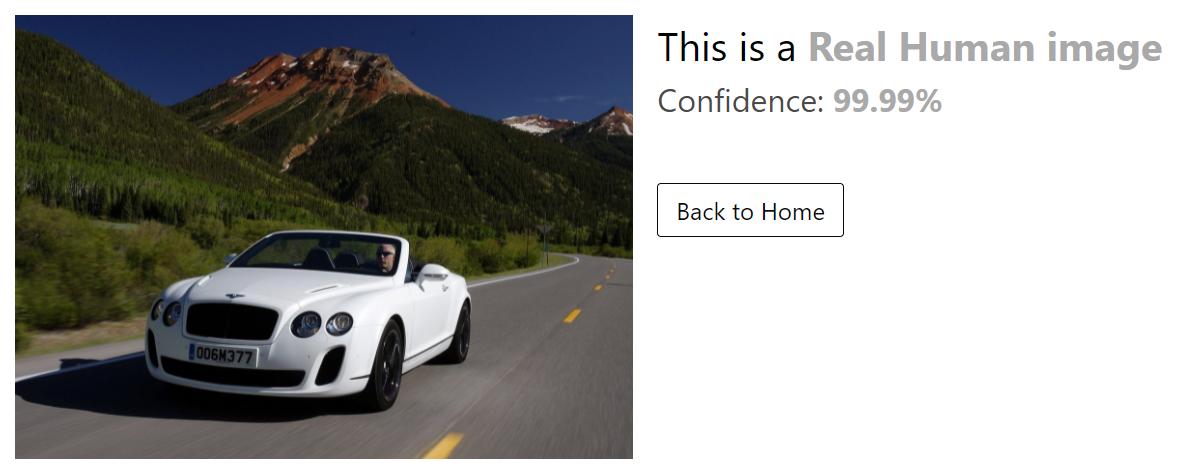
\includegraphics[width=0.7\textwidth]{img/f11.png}}%
\caption{Acceptable level of Overfitting for the StyleGAN identification model}%
\label{fig:11}%
\end{figure}
  
A subset of these 2 datasets will improve the development of the artefact as working with a large dataset while testing and implementing hot and cold learning will unnecessarily increase the development time. Training times are influenced by the number of epoch in training and the number of samples used. When developing a neural network works it is standard to use a small subset of the training set to keep the times in testing lower, and after the development of the neural network is completed move over to the full dataset. The Full dataset that will be used in the final training and optimization of the neural network will be larger than the small dataset used in development to ensure that the final model can identify the features present in StyleGAN generated images. Table \ref{tab:sizes} states the sizes of the datasets and the subdirectories that will be used in the development and the final optimization of the neural network model. 

\begin{table}[H]
\caption{Total amount of images used in the Artefact creation}
\label{tab:sizes}
\resizebox{\textwidth}{!}{%
\begin{tabular}{lllllll}
\hline
Directory & \multicolumn{2}{c}{Development} & \multicolumn{2}{c}{Training} & \multicolumn{2}{c}{Optimization} \\ \hline
\multicolumn{1}{|l|}{} & \multicolumn{1}{c|}{sg} & \multicolumn{1}{c|}{ff} & \multicolumn{1}{c|}{sg} & \multicolumn{1}{c|}{ff} & \multicolumn{1}{c|}{sg} & \multicolumn{1}{c|}{ff} \\ \hline
\multicolumn{1}{|l|}{Train} & \multicolumn{1}{l|}{1000} & \multicolumn{1}{l|}{1000} & \multicolumn{1}{l|}{2000} & \multicolumn{1}{l|}{2000} & \multicolumn{1}{l|}{4000} & \multicolumn{1}{l|}{4000} \\ \hline
\multicolumn{1}{|l|}{Validation} & \multicolumn{1}{l|}{500} & \multicolumn{1}{l|}{500} & \multicolumn{1}{l|}{1000} & \multicolumn{1}{l|}{1000} & \multicolumn{1}{l|}{2000} & \multicolumn{1}{l|}{2000} \\ \hline
\multicolumn{1}{|l|}{Test} & \multicolumn{1}{l|}{500} & \multicolumn{1}{l|}{500} & \multicolumn{1}{l|}{1000} & \multicolumn{1}{l|}{1000} & \multicolumn{1}{l|}{2000} & \multicolumn{1}{l|}{2000} \\ \hline
Total Dataset Size &  & 4000 &  & 8000 &  & 16000 \\ \hline
\end{tabular}%
}
\end{table}

Table \ref{tab:sizes} and Table \ref{tabl:folders} shows the layout of the directories that must be consistent throughout the training of the neural network model in the artefact creation. In binary image classification, the process of training a neural network to classify two sets of images into two separate classes, the neural network references the directory in which an image resides for its check on its prediction. This means that in the training stages the neural network will make its prediction on an image, and check if that image is in the real human directory (ff) or the StyleGAN generated images directory (sg) and then change its weights according to the correlation between its prediction and the directory path of the image receives. In short, the neural network will use the directories to "\textit{know}" what type of image the received training image is. 

The validation folder in the directory is the set of images the neural network uses to check its accuracy after each training step while training its weights. The neural network changes its weights after each image in the training set and just uses the validation set as a benchmark for each checkpoint in training. The Test set is important as it will be used to evaluate the final model. The Test set must be kept aside and never accessed in the training phase of the model. Thus a Test set was created early with unique images the will not be accessed again in the training phases.

\subsubsection{Creating the First Neural Network}

For the creation of the Artefact, it was identified that the problem of identifying StyleGAN generated images required binary image classification. To understand how binary image classification could be applied to a StyleGAN problem the Cat-vs-Dog example was used to understand binary image classification. The Cat-vs-Dog problem can be seen as a Hello World exercise that will teach the base fundamentals of binary image classification and the knowledge gained in this problem will be applied to the StyleGAN problem \citep{cat2014}. The Cat-vs-Dog problem is a basic exercise to create a neural network to classify images as either a cat or a dog, and the dataset used in this exercise contains 4000 images of both cats and dogs with image sizes of 200px by 200px. 

The StyleGAN problem was applied to this exercise by using the StyleGAN dataset instead of Cat-and-Dog images. A problem was identified with this implementation as StyleGAN images are very large compared to other datasets used in CNN neural network implementations, namely the MINST handwriting dataset and the Cat-vs-Dog dataset. StyleGAN images and FlickrFaces images native resolution is 1024px by 1024px, which could not be passed to a neural network catered for the classification of Cat-vs-Dog images as the input layer of the neural network must match the image resolution in CNN's \citep{cat2014, Wang}. Figure \ref{fig:13} shows the input layers and image sizes in identifying StyleGAN images and the Cat-vs-Dog exercise.

\begin{figure}[H]%
\centering
\fbox{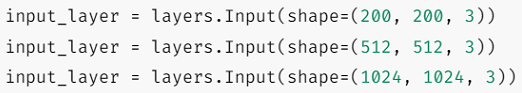
\includegraphics[width=0.95\textwidth]{img/f13.png}}%
\caption{Input layer of the neural network according to the image sizes}%
\label{fig:13}%
\end{figure}

In Figure \ref{fig:12} a comparison between a dog image retrieved from the Cat-vs-Dog dataset and the dataset used for the identification of StyleGAN images in this project with the sizes of the original images (1024x1024px) the scaled-down (200x200px) images to fit into the input layer of the Cat-vs-Dog problem. 

\begin{figure}[H]%
\centering
\fbox{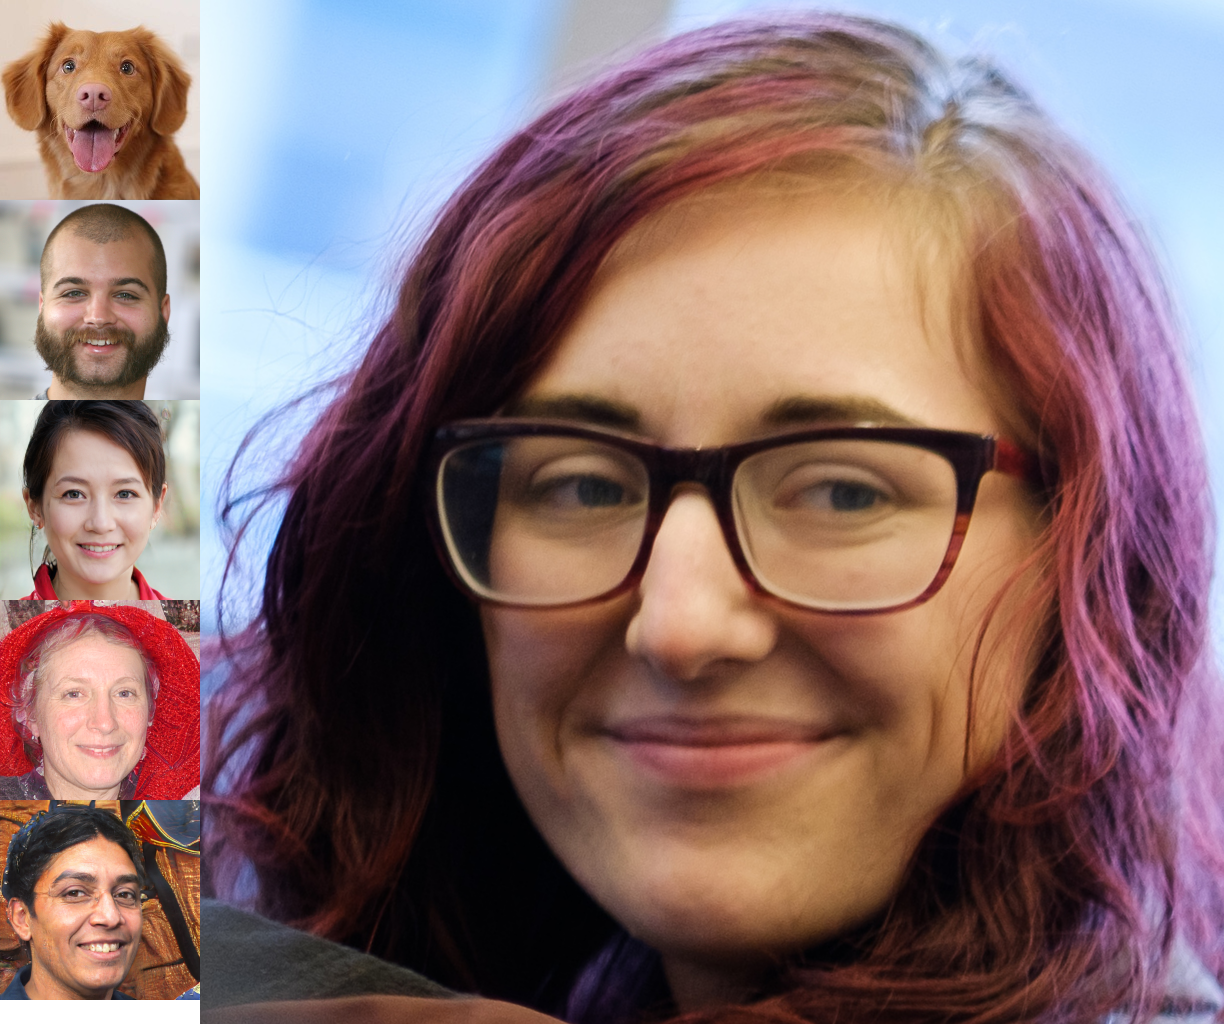
\includegraphics[width=0.9\textwidth]{img/f12.png}}%
\caption{Image sizes of Cat-vs-Dog dataset, rescaled artefact dataset and StyleGAN original sizes}%
\label{fig:12}%
\end{figure}

When the StyleGAN images were passed into the Cat-vs-Dog neural network with a change in the input layer of the network to accommodate full resolution StyleGAN images a usage limit was reached on Google Colab. This identified that some image processing will be required on the dataset. When the images were scaled down to 200x200px and the Cat-vs-Dog neural network trained on StyleGAN images an accuracy of 61\% was achieved. The accuracy achieved with this basic implementation was used as a proof of concept and showed that it was possible to identify StyleGAN images with a neural network. The accuracy of the network however was not ideal and thus a network specific to the StyleGAN problem had to be created.

\subsubsection{Image Processing}

As mentioned in the previous section, the dataset of images gathered for the identification of StyleGAN images had to be processed to allow the neural network to train on these images. Image processing is an entire field on its own with theory relating to it. For the image processing needs to be required in this stage of the artefact development the python library OpenCV was identified to be the simplest solution to the problem being faced. 

OpenCV is a programming library geared mostly at real-time computer vision. It was created by Intel and then supported by Willow Garage and Itseez. Under the open-source Apache 2 License, the library is cross-platform and free to use \citep{opencv2012}. A python script was created to change the entire dataset sequentially and the need to manually scale the image was avoided. The script was used to create different datasets for later use in this proposed project. The image resolutions of the different datasets created included a 200x200 pixels, 512x512px and 1024x1024px.

%too many trainable parameters
%take too long exhaust resources
%the more data the better but nn can work with little

\subsubsection{Summary}

The first sprint in the development of the artefact required the dataset to be retrieved, structured and the images processed. The dataset was downloaded using the rclone program to avoid the throttling limitation experienced. The layout of the directories in the dataset that was compiled for the identification of StyleGAN images was structured to enable the dataset to be used in training. The Cat-vs-Dog exercise proved that a StyleGAN identification neural network model could be created and showed that images had to be processed for a neural network to be trained on the limited resources available. For the processing of the images, a python script was created using the open-source image processing library OpenCV.

\subsection{Sprint 2}
 
In the second sprint of the artefact development, the first neural network was created based on the findings in the first sprint and using that dataset gathered and processed in the first sprint. The initial neural network that was created in this phase of the artefact development just required hot and cold learning and was not optimized in any form. Hot and Cold learning as analysed in Chapter \ref{ch1} is an uninformed guessing game in hyperparameter optimization.

\subsubsection{Creating the First Neural Network}

To create the neural network the TensorFlow package was used. TensorFlow is a machine learning and artificial intelligence software library that is free and open-source. It may be used for a variety of applications, but it focuses on deep neural network training and inference \citep{tensor2016}. TensorFlow was used within the Jupyter Notebooks in Google Colab and locally, and was run in the python environment.

 Keras is an open-source software library for artificial neural networks that include a Python interface \citep{kerascnn2017}. Keras serves as a user interface for TensorFlow. Keras supports the TensorFlow package and is used for creating the neural network in the development of the artefact \citep{kerascnn2017}.
 
The initial neural network was then created using TensorFlow and Keras in Google Colab. The Code for the notebooks used can be found in Appendix \ref{AppendixC} and \ref{AppendixD}. As seen in Figure \ref{fig:nn1} the neural network consisted of 3 convolutional layers, a single dense layer and had a total amount of trainable parameters exceeding 17 million. The large amounts of trainable parameters would result in the resources available in Google Colab being exhausted in training. A hot and cold learning approach was taken and with the smaller test dataset, the model was trained and changed until some improvements could be seen. The trained accuracy of this neural network was 51\% at this stage but could be improved more. 

\begin{figure}[H]%
\centering
\fbox{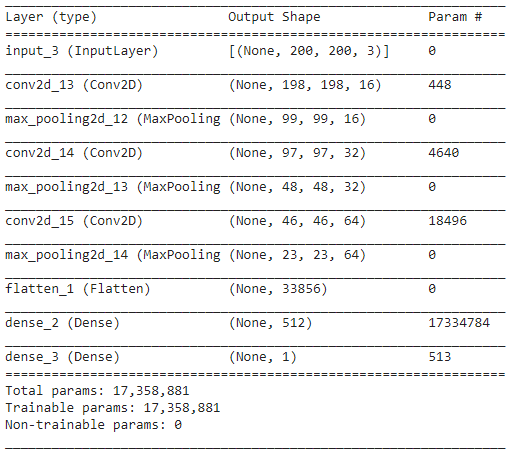
\includegraphics[width=0.65\textwidth]{img/fnnarch1.png}}%
\caption{Summary of Cat-vs-Dog network applied to the StyleGAN problem}%
\label{fig:nn1}%
\end{figure}

More layers and dropout layers were added to the different convolutions using hot and cold learning. Figure \ref{fig:nn2} is a summary of the neural network architecture of a model created for the identification of StyleGAN images using the principles of hot and cold learning applied on the hyperparameters of the model.  

\begin{figure}[H]%
\centering
\fbox{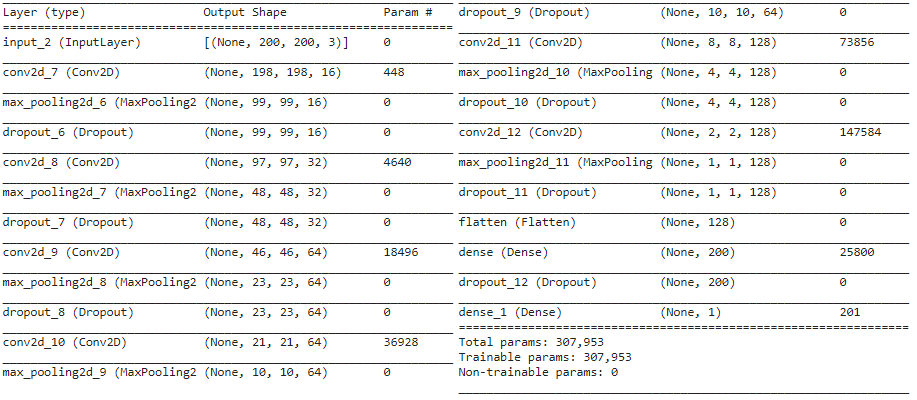
\includegraphics[width=0.95\textwidth]{img/nn2.png}}%
\caption{Summary of the created Neural Network}%
\label{fig:nn2}%
\end{figure}

The final self-created neural network trained on the training dataset could identify the StyleGAN generated images with 81\% accuracy using the test data. The relatively high true accuracy showed promising results but because of the randomness in hot and cold learning and what was identified in the literature review of Chapter \ref{ch2}, the hyperparameters had to be optimized.


\subsection{Sprint 3}

Hot and Cold learning is a viable option for setting neural network parameters when developing neural networks and learning how they can be used to solve problems \citep{Trask2019}. But for the identification of StyleGAN images hot and cold learning proved to be an inefficient manner in which to create the neural network architecture. Optuna was defined as a possible technology to omit the hot and cold learning process and create a highly optimized neural network.  

\subsubsection{Optuna: A hyperparameter optimization framework}

Optuna is a software framework for automated hyperparameter optimization that is specifically developed for machine learning. It has an imperative, define-by-run user interface. The code built with Optuna has a high level of flexibility thanks to its define-by-run Interface, and the user of Optuna may dynamically design the search spaces for the hyperparameters. The phrases "study" and "trial" are used as follows: A Trial is a single execution of the objective function, whereas a Study is optimization based on an objective function \citep{optuna2019}.

When the Optuna hyperparameter process was started in this sprint the trail function and study functions were created based on the documentation of the Optuna framework. The trail is a single iteration in the larger study and the study is a collection of trails where different combinations of hyperparameters are used to reach the goal of the trail. The study goal for identifying StyleGAN images was to increase the accuracy and \cite{optuna2019} terms it was to move the accuracy metric in a maximum position. The trail function was set to suggest a neural network layer count ranging from a single layer network to a 7 layer network. The optimizer was suggested from a pool of optimizers that perform well with image classification problems as was identified by \cite{bera2020analysis} and \cite{kandel2020comparative}. The Study could be changed to also train full neural networks on each trail but it was decided to train the networks the minimal amount just to evaluate the improvements of the models. When the study was completed the resulting model was then trained on the full dataset.

When the Optuna study was executed on Google Colab a problem was faced regarding available resources. Google Colab provides a free service but can throttle users resources based on the amount of resources used. The policies that Google use to dictate what will amount to throttling is unclear and Google can throttle any account based on their discretion. When the Optuna study started the account used on Google Colab for the development of the artefact was throttled down and exceeded the acceptable usage dictated by Google. To work around the problem the jupyter notebooks was downloaded and run on a physical computer provided by Prof. Tiny du Toit. The computer used for the study included a GPU, namely a GTX 1080 with 8GB dedicated graphics memory.

\textbf{Graphics cards differences: compare collab and Nvidia gpu}

\textbf{Image of Optuna output in Study}

\textbf{Train}

\textbf{Image of training}

The model created using the Optuna framework for hyperparameter optimization was trained on the full dataset on the local machine as previously stated and training times were increased due to the improved machine learning factor of the improved GPU. The trained hyperparameter optimized model could identify StyleGAN generated images with an accuracy of 97.3\% and true accuracy of 97.6\% as tested with the python script. The results of the Optuna network compared to the network created in Sprint 1 will be further discussed in the Results chapter in this document.


\subsection{Sprint 4}

With the neural network model completed and trained to exceptional accuracy, a front-end application was created to allow users to easily and intuitively interact with the model as stipulated as one of the objectives of this project. By allowing users to interact with the model easily the aim of identifying StyleGAN images can be satisfied as users will be able to pass images to the neural network that in turn will be able to identify if these images were generated by StyleGAN or if the images are that of real human beings. 

For the front end of the artefact a web application, that will allow for easier deployment and wider reach had to be created to satisfy the objectives of this proposed project. In the final sprint of the artefact development, various frameworks were considered and while developing the artefact it was realised that a python-based web framework will enable the implementation of the neural network. 

\subsubsection{Adding the model to the Web App}

Because the neural network model was created using the Python libraries for machine learning it was realised that a python-based framework will allow the neural network to be implemented in the web app. If another front end framework like React or Angular was used the implementation of the neural network would be unnecessarily complex. React and Angular are JavaScript based frameworks and for the Python model to communicate with the front end of a JavaScript framework an API had to be implemented. The neural network requires the python machine learning libraries TensorFlow and Keras to pass an image through the model and provide the identification as feedback. Thus the libraries must reside in a python environment where TensorFlow and Keras are installed. 

To avoid this added complexity an analysis into python web-based frameworks where conducted and the Django framework stood out. The Django framework however is a very large and clunky framework when compared to the implementation required for the artefact. The child framework Flask, which was derived from Django but with a lightweight footprint was used for the creation of the front-end of the artefact. The Flask app was developed as a minimalistic interface that would guide users intuitively on how to use the app with clear instructions and a simplified design. 

python requires backend

we use TensorFlow and Keras

Django

flask better

artefact looks

home page

UI UX error and 404 

Identified StyleGAN

Identified FF



\section{Summary}